\chapter{Concept}
\label{chap:concept}

This chapter describes the novelty that you have created during the making of your thesis.
This novelty might be an experimental apparatus, a novel algorithm, or a thorough analysis of something.
You may here reuse the background information presented in the previous chapter.

\section{Figures in Latex}
\Cref{fig:excitation-contraction-coupling} shows experimental measurements of the excitation-contraction coupling in human skeletal muscles.
Note the extensive figure caption: many readers will first skim through your thesis and look at the figures, which should hence be as self-explanatory as possible.
\begin{figure}
  \centering
  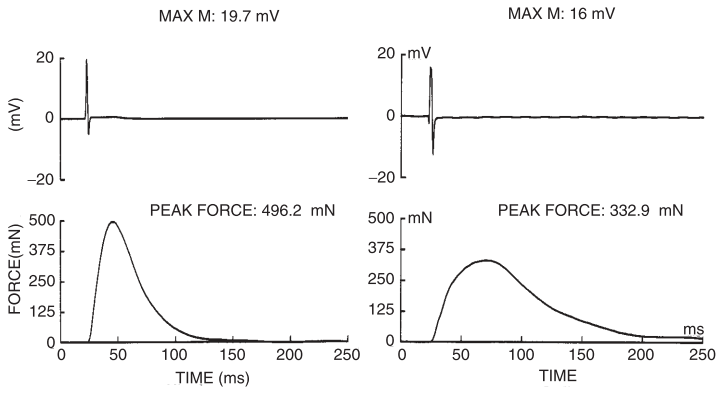
\includegraphics[width=12cm]{excitation-contraction-coupling}
  \caption[Measurements of the excitation-contraction coupling for exemplary fast-twitch and slow-twitch muscle fibres]{Measurements of the excitation-contraction coupling for exemplary fast-twitch (left) and slow-twitch (right) muscle fibres. Shown are the electrical (top) and mechanical (bottom) signals generated during a single fibre contraction. Note the discrepancy in time scales. (Reprinted from \cite{merletti04})}
  \label{fig:excitation-contraction-coupling}
\end{figure}

As opposed to \cref{fig:excitation-contraction-coupling}, which is included here as an external graphics file, \cref{fig:simple-schematic} shows a simple electrical schematic that is created completely in Latex, using the \swname{circuitikz} package.
\begin{figure}
  \centering
  \begin{circuitikz} \draw
    (0,0) to [V=$U_0$] (0,3)
    to [R=$R_I$, i=$I_R$] (3,3)
    to [R=$R_L$] (3,0)
    to [C=$C_P$] (0,0)
    ;
  \end{circuitikz}
  \caption{A simple electrical circuit, drawn in Latex using the \swname{circuitikz} package.}
  \label{fig:simple-schematic}
\end{figure}
This package is based on the powerful \swname{tikz} package which allows for drawing any kind of figure directly in Latex.
This bears a number of advantages:
\begin{itemize}
\item The resulting figures are vector graphics, i.e., they are small (hence not resulting in a final thesis pdf size of several MBs) and generally look good.
\item Font style and size is consistent with the rest of the document. This is a major problem when importing figures from other software, e.g., \swname{Matlab}.
\item Each figure created this way is completely reproducible and configurable in every aspect.
\end{itemize}
Another package that is also based on the \swname{tikz} package is the \swname{pgfplots} package which enables the user to create plots either completely in Latex, or import data from an external program (e.g., \swname{matlab}) and generate a nice-looking plot from this data using \swname{tikz} (with the advantages mentioned above).
\Cref{fig:rosenfalck} shows an example of two plots generated using the \swname{pgfplots} package.
\begin{figure}
  \centering
  \newcommand*{\scalefactor}{0.8}
  \begin{subfigure}[t]{.5\textwidth}
    \centering
    \begin{tikzpicture}
        \newcommand*{\Aros}{96}
  \newcommand*{\Bros}{-90}
  \begin{axis}[
    small,
    width = \scalefactor\textwidth,
    axis lines = left,
    x unit = mm,
    y unit = mV,
    xlabel = $z$,
    ylabel = $V$,
    xtick={0,5,10},
    ymin = -99,
    ymax = 49,
    extra y ticks = {\Bros},
    extra y tick labels = {$B$},
    ]
    % Right part of the expression
    \addplot [
    domain=-2:15, 
    samples=1000, 
    color=blue,
    ]
    {x>0 ? \Aros*x^3*e^(-x)+\Bros : \Bros};

    \draw[dashed] (-2,\Bros) -- (15,\Bros);
  \end{axis}
    \end{tikzpicture}
    \caption{$V_m(z)$}
    \label{fig:rosenfalck-1}
  \end{subfigure}%
  \begin{subfigure}[t]{.5\textwidth}
    \centering
    \begin{tikzpicture}
      \newcommand*{\Aros}{96}
\newcommand*{\Bros}{-90}
\pgfplotsset{set layers}
\begin{axis}[
  small,
  width = \scalefactor\textwidth,
  axis y line = left,
  axis x line* = bottom,
  x unit = mm,
  y unit = mV/mm,
  xlabel = $z$,
  ylabel = $\psi$,
  xmin = -15,
  xmax = 2,
  ymin = -79,
  ymax = 39,
  xtick = {-10, -5, 0},
  ]

  \addplot [
  domain=-15:2, 
  samples=1000, 
  color=blue,
  ]
  {x>=0 ? 0 : -3*\Aros*x^2*e^x-\Aros*e^x*x^3}
  node[pos = 0.03,
       pin = 70 : {$\psi$}] {};

\end{axis}

\begin{axis}[
  small,
  width = \scalefactor\textwidth,
  axis y line = right,
  axis x line = none,
  x unit = mm,
  y unit = mV/mm^2,
  xlabel = $z$,
  ylabel = $\psi'$,
  xmin = -15,
  xmax = 2,
  ymin = -59,
  ymax = 119,
  ]

  \addplot [
  domain=-15:2, 
  samples=1000, 
  color=purple,
  ]
  {x<0 ? -(6*x+6*x^2+x^3)*\Aros*e^x : 0}
  node[pos = 0.02,
       pin = 70 : {$\psi'$}] {};
\end{axis}                      

    \end{tikzpicture}
    \caption{$\psi(z)=\dd{z} V_m(-z)$ and $\psi'(z)$}
    \label{fig:rosenfalck-2}
  \end{subfigure}%
  \caption[Plots of Rosenfalck's model function for the \acrlong{iap}]{Plots of the \acrfull{iap} model function proposed by \textcite{rosenfalck69}.}
  \label{fig:rosenfalck}
\end{figure}

\section{Blind Source Separation Methods}
In this chapter in particular, you should provide a lot of references, e.g., to scientific articles~\cite{farina99}, books~\cite{plonsey07}, book chapters~\cite{rodriguez-falces12}, PhD theses~\cite{fevotte03}, or software projects~\cite{r-project} that you used during the creation of your thesis.
Sometimes, you should explicitly name authors, such as \textcite{farina99}, who wrote a seminal article on the mathematical modelling of \gls{emg} measurements.

Note how the \gls{emg} acronym is clickable and leads to the definition of this acronym in the glossary.
This is one of the many features of the \swname{glossaries} package.

\subsection{Equations}
If you are going to write more than a few equations in your thesis, it is highly recommendable to use macros to define each variable that occurs.
This way, if you decide to rename the velocity from $v$ to $v_0$ everywhere in your thesis later on during the process of writing, you will only have to change the definition of the macro used for this variable.
For example, in
\begin{equation}
  \label{eq:1}
  \vel = \frac{\diff \loc}{\diff t}
\end{equation}
and
\begin{align}
  \label{eq:2}
  \acc &= \frac{\diff \vel}{\diff t} \nonumber \\
  &= \frac{\force}{\mass}
\end{align}
each of the variables is defined using a macro.
Finally, here comes an example of how to reference equations \eqref{eq:1} to \eqref{eq:2}.

\section{Pseudo Code}
Algorithm \ref{alg:intexp} is an example of how pseudo code can be represented in Latex.
Of course there are, as with anything in Latex, many options available to achieve this goal.
Here, the \swname{algorithmic} package is employed.
\begin{algorithm}
  \begin{algorithmic}
    \FORALL{muscle fibres $i$}
    \FORALL{electrodes $j$}
    \STATE evaluate $\Bfun_{i,j}(k_z)$ at a set of points $k_{z,n}$
    \STATE initialise $\Bfun_{i,j,\text{interp}}(k_z)$, an interpolation / extrapolation of $\Bfun_{i,j}(k_{z,n})$
    \FORALL{temporal frequencies $k_{t,m}$ required for the inverse Fourier transform}
    \STATE calculate $\Afun_{i,j}(k_{t,m})$, using $\Bfun_{i,j,\text{interp}}(k_z)$ instead of $\Bfun_{i,j}(k_z)$
    \ENDFOR
    \ENDFOR
    \ENDFOR
  \end{algorithmic}
  \caption{Algorithm for the efficient numerical evaluation of $\Afun_{i,j}(k_{t,m})$.}
  \label{alg:intexp}
\end{algorithm}


%%%%% Emacs-related stuff
%%% Local Variables: 
%%% mode: latex
%%% TeX-master: "../../main"
%%% End: 
